%% File 'sample.tex'
%% 
%% Copyright (C) 2003 by Maarten Sneep <sneep@nat.vu.nl>
%% Modified 2004 by B.Ph. van Milligen <boudewijn.vanmilligen@ciemat.es>
%% 
%% This file may be distributed and/or modified under the conditions of
%% the LaTeX Project Public License, either version 1.2 of this license
%% or (at your option) any later version.  The latest version of this
%% license is in:
%% 
%%    http://www.latex-project.org/lppl.txt
%% 
%% and version 1.2 or later is part of all distributions of LaTeX version
%% 1999/12/01 or later.
%% 
\documentclass{epsconf}
\usepackage{graphicx}
%\usepackage{epsfig} % use this package to include EPS format figures
\usepackage{wrapfig}
\usepackage{amsmath}
\usepackage{amssymb}
\newcommand{\bb}[1]{\textbf{#1}}

\title{Dependence of the Nonhelical Dynamo on Shear: Numerical Exploration of the Magnetic Shear-current and Stochastic-$\alpha$ Effects}
\author{\underline{A. Hankla}$^1$, C. Fendt$^1$}
\institute{$^1$ Max Planck Institute for Astronomy, Heidelberg, Germany}

\begin{document}
\maketitle

\section{Introduction}
Accretion disks are ubiquitous in astrophysical systems, ranging in scales from propoplanetary disks around stars to disks around active galactic nuclei (AGN). When the disk is mostly ionized and threaded by a weak magnetic field, the magnetorotational instability (MRI) leads to radially-inward transport of angular momentum~\cite{bh91}. At its heart, the MRI is a shear-driven instability: the importance of shear was therefore explored early on, exposing numerical and analytical evidence for how various quantities scale as a function of shear~\cite{abl96}.

However, some of these previous works may have cut out important physics due to numerical constraints that limit the simulation regime to a locally Cartesian ``shearing box". In particular, a small vertical height can artificially dampen a large-scale dynamo~\cite{SSH16}. With box sizes in mind, we recreate previous results in small boxes but in larges boxes uncover an abrupt (previously unreported) jump in how various quantities scale with shear that we suspect to be connected to the presence/absence of a large-scale dynamo. 

This study focuses on unstratified systems, whose additional reflectional symmetry means that the dynamo presence cannot by explained by the well-known $\alpha$-effect. We explore two alternatives: the magnetic shear-current effect, an analog to the kinematic shear-current effect fueled by a negative off-diagonal diffusivity~\cite{SB16}, and the stochastic-$\alpha$ effect, which drives the dynamo through fluctuations in the $\alpha$ parameter that average to zero over an ensemble of many initial conditions~\cite{hms11}. Comparison of these two models is facilitated by explicitly calculating transport coefficients and adjusting the simulation domain size XX. We note that, unlike for the so-called ``butterfly diagrams" of $\alpha\Omega$ dynamos~\cite{GP15}, there is currently no analytic derivation for the cycles of the mean azimuthal magnetic field in an unstratified dynamo: we therefore provide preliminary scalings to motivate future analytic research.

Although accretion disks are in general vertically stratified, the midplane region of the disk is roughly unstratified. Therefore we can compare our results to the inner portion of previous studies' stratified shearing boxes. Unstratified boxes have the added advantage of isolating specifically nonhelical dynamo mechanisms.

\section{Methods} 
The basis of this project is solving the ideal compressible single-fluid magnetohydrodynamic (MHD) equations within the unstratified shearing box approximation. This is done by using the $\texttt{ATHENA}$ code with the CTU integrator, Roe Riemann solver, and the FARGO orbital advection scheme~\cite{StoneGardiner2010}. The equations solved are:
\begin{align}
    \frac{\partial\rho}{\partial t}+\nabla\cdot(\rho\bb{v})=0, &\hspace{.5in}  \frac{\partial\bb{B}}{\partial t} - \nabla\times(\bb{v}\times\bb{B})=0, \\
    \frac{\partial\rho\bb{v}}{\partial t} + \nabla\cdot(\rho\bb{vv}+\bb{T})&= -2\rho\Omega\hat z\times\bb{v}+2q\rho\Omega^2~x\hat x,
\end{align}
where $\bb{T} = \left(P+\frac{\bb{B}\cdot\bb{B}}{8\pi}\right)\bb{I}-\frac{\bb{BB}}{4\pi}$ is the total stress tensor. As usual, $\rho$ is mass density, $\bb{v}$ is the plasma velocity, and $\bb{B}$ is the magnetic field. Here, the disk is rotating with angular frequency $\Omega\hat z$, and $\hat x$ is the radial direction. We focus on varying the shearing parameter $q$, defined through $\Omega\sim r^{-q}$ as $q\equiv-d\ln\Omega/d\ln r$. Hence $q=3/2$ corresponds to the familiar Keplerian rotation profile.

Simulations are run with an adiabatic equation of state with a box size of $[L_x,~L_y,~L_z] = [1,~4,~4] H$, where $H$ is the disk scale height, and resolution of 64, 128, and 256 zones, or 64, 32, and 64 zones/$H$, unless otherwise stated. The initial magnetic field is $\bb{B}=B_0\sin(2\pi x/L_x)\hat z$ (zero net flux) with $B_0$ defined via the plasma beta parameter $\beta = 8\pi P_0/B_0^2 = 4000$. 

To make contact with the magnetic shear-current model, we calculate the transport coefficients that come out of mean field theory: after assuming scale separation between the large-scale mean field and the small-scale turbulent field $\mathbf{B_T}=\bar{\bb{B}}+\bb{b}$ where the volume average (denoted by $\langle\cdot\rangle$) of the turbulent field $\langle\bb{b}\rangle=0$, the mean field portion of the induction equation becomes
\begin{align}
    \frac{\partial\bar{\bb{B}}(z)}{\partial t}&=\nabla\times\left[\bb{v}(z)\times\bar{\bb{B}}(z)+\mathcal{E}(z)-(q\Omega x\hat y)\times\bar{\bb{B}}(z)\right] \label{eq:mind}
\end{align}
where $\mathcal{E}=\langle \bb{v}\times\bb{b}\rangle$ is the mean electromotive force. Scale-separation arguments allow Taylor-expanding $\mathcal{E}$ in terms of $\bar{\bb{B}}$: $\mathcal{E}_i = \alpha_{ij}\bar{B}_j - \eta_{ij}(\nabla\times\bar{B})_j$ where we have used $B_z = 0$ and that the mean field depends only on the $z$-direction. To directly calculate the dynamo transport coefficients $\alpha$ and $\eta$, we employ the projection method, calculating $\mathcal{E}$, $\bar{\bb{B}}$, and $\partial_z\bar{\bb{B}}_i$ from simulation data, computing $\langle\mathcal{E}_iM\rangle$ for each $M\equiv(\bar B_x, \bar B_y, \partial_z\bar B_x, \partial_z\bar B_y)$, and solving Eq.~\ref{eq:mind}'s resulting matrix equation in the least-squares sense at each time step. We impose the constraints $\alpha_{xx}=\alpha_{yy}$, $\alpha_{yx}=0=\eta_{xy}$, and $\eta_{xx}=\eta_{yy}$ for cleaner results~\cite{SB16}. 

\section{Results}
\begin{wrapfigure}{r}{0.6\textwidth}
\vspace{-1cm} \begin{center}
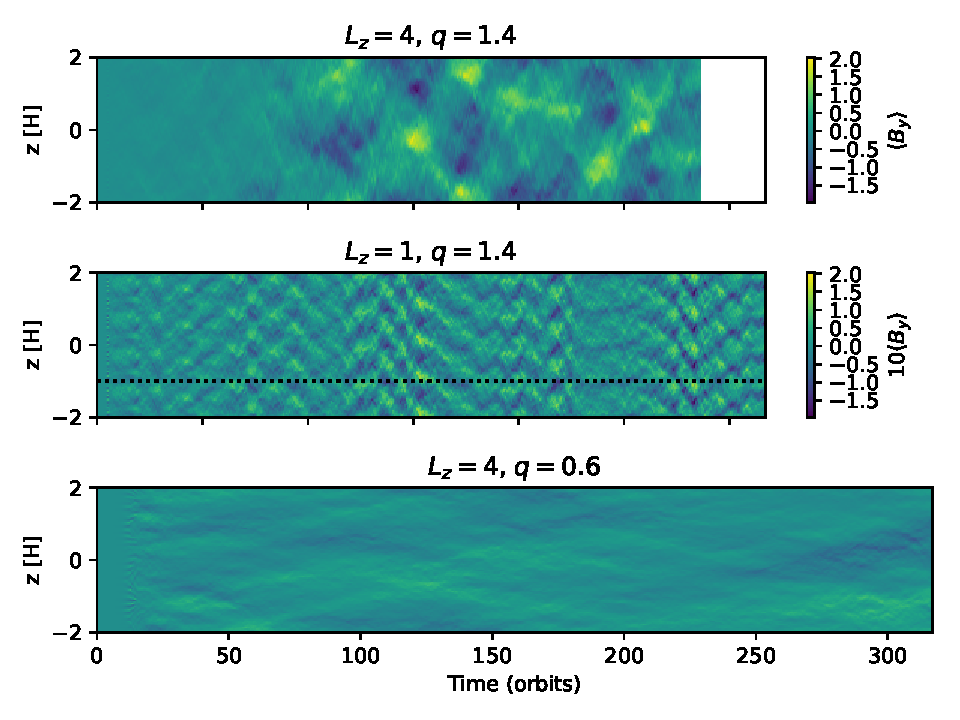
\includegraphics[width=\linewidth]{fig_xyazte_butterfly_compare_qz.pdf}
\caption{\it \small The small box has been duplicated 4 times to have the same aspect ratio. Dotted black line shows the actual simulated domain. Color bar is the same for middle and bottom.}
\label{fig:butterfly}
\end{center} 
\vspace{-1cm}
\end{wrapfigure}%
We first seek to show that a large-scale dynamo is indeed present. Convincing evidence for a large-scale magnetic field comes from the mean azimuthal magnetic field as a function of height and time. We compare a tall box with $q>1.2$ (top), a small box (middle), and a tall box with $q<1.2$ (bottom) in Fig.~\ref{fig:butterfly}. The tall box with dynamo action has patches of magnetic field that are on the order of $H$, whereas the small box/low $q$ do not.

Dynamo action also manifests in volume-averaged quantities such as the ratio of mean to turbulent magnetic field energy (Fig.~\ref{fig:mtbr}). For small values of $q$, the mean energy is only about one-fifth of the turbulent field energy. The jump at $q\gtrapprox1.2$ could indicate a dynamo switching on, since the mean and turbulent fields contribute approximately equally to the total mean energy.
\begin{figure}[h]
\vspace{0cm}
\begin{minipage}{0.48\textwidth}
    \centering
    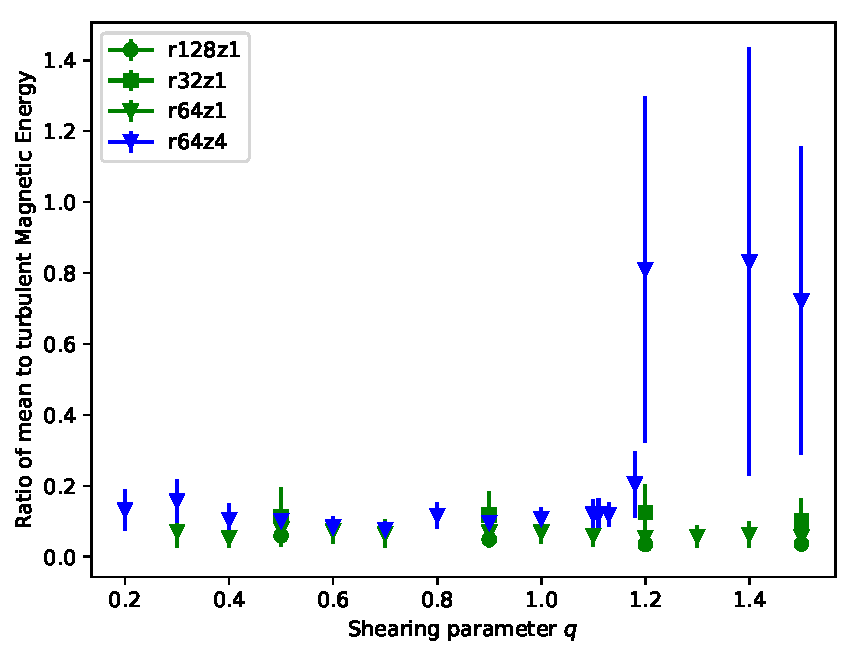
\includegraphics[width=\linewidth]{fig_vata_mtT_MEmtr_err.pdf}
    \caption{\it \small Runs with varying resolution (denoted by $r$: $r32$ corresponds to 32 zones/$H$) and box height ($z1$ being $L_z=1$).}
    \label{fig:mtbr}
\end{minipage}%
\hfill%
 \begin{minipage}{.48\textwidth}
  \centering
    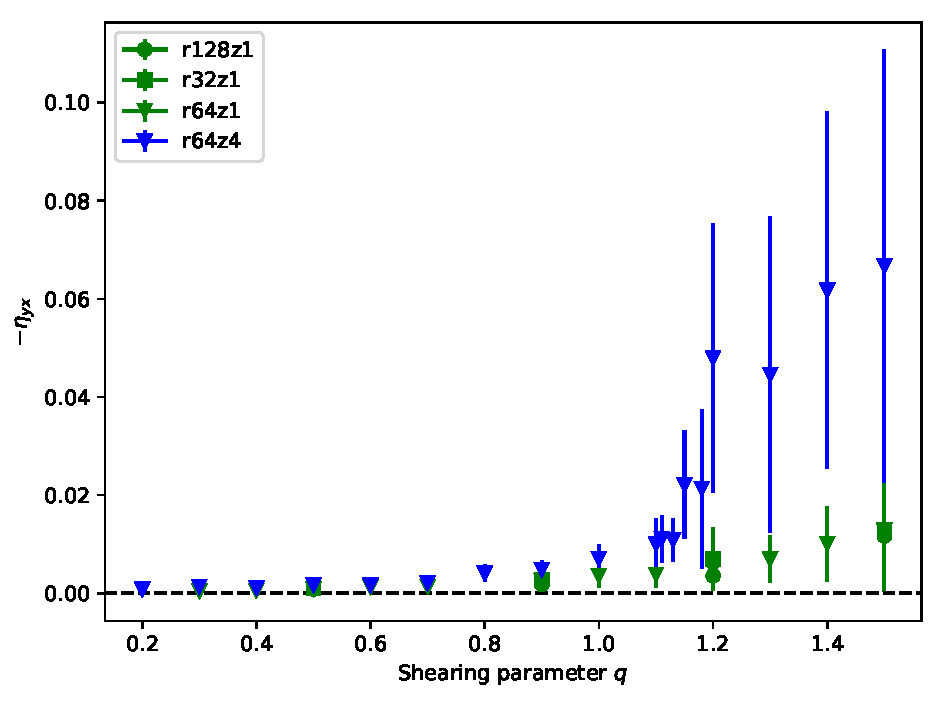
\includegraphics[width=\linewidth]{fig_vataqe_etayx_const_t100-end_hgbLAIF_err.pdf}
    \caption{\it \small Averaged over $t=100-200$ orbits, the saturation period. Black dotted line is at zero. Error bars indicate one standard deviation. }
    \label{fig:etayx}
\end{minipage}
\vspace{0cm}
\end{figure}
To investigate whether this break is related to a potential dynamo mechanism, we calculate the transport coefficients as a function of shear. We are particularly interested in the off-diagonal component $\eta_{yx}$, which, when negative, is the hallmark of the magnetic shear-current effect. Indeed, as seen in Fig.~\ref{fig:etayx}, this coefficient is negative for all simulations, abruptly jumps at the same $q\approx1.2$, and has the same behavior with box size as in Fig.~\ref{fig:mtbr}. As a check, the $\alpha$ coefficients average to zero. A toy model attempting to explain the cycles of Fig.~\ref{fig:butterfly} through a sign change in $\eta_{yx}$ when the azimuthal field reaches a critical value~\cite{LesurOgilvie08} is not supported because the coefficient remains negative throughout our simulations. To guide future explanation attempts, Fig.~\ref{fig:qperiod} presents azimuthal field cycle periods, calculated by fitting the largest vertical mode at a given $z$~\cite{SSH16}. 
\begin{wrapfigure}{l}{0.48\textwidth}
\begin{center} \vspace{-1cm}
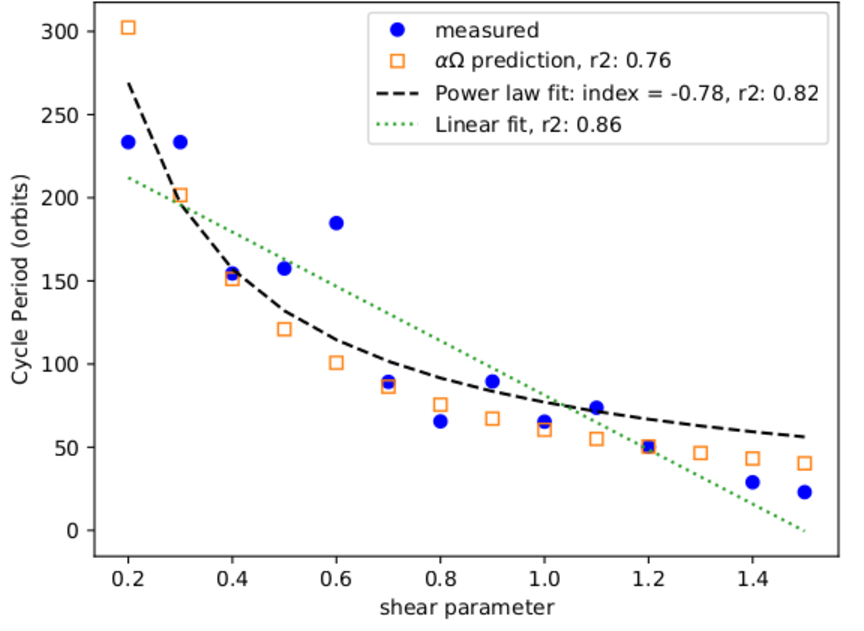
\includegraphics[width=\linewidth]{fig_q_cycle_period_hgbLAIF_r64z4b4000znf.pdf}
\caption{\it \small Comparison of $\alpha\Omega$ scaling relation period $T\sim 1/q$ and linear and power-law fits~\cite{GP15}.}
\label{fig:qperiod}
\vspace{-1cm}
\end{center}
\end{wrapfigure}
The stochastic-$\alpha$ effect manifests through a change in dynamo growth rate when the horizontal domain size is changed. We find XXX

\section{Conclusions}
We have presented preliminary evidence for the presence of the magnetic shear-current effect in large, unstratified shearing boxes. Future work includes examining boxes with $L_z\approx8$ where clearer trends should emerge, running multiple initial conditions to better understand the impact of the stochastic-$\alpha$ effect, and including explicit dissipation. 
\section{Acknowledgments}
This project was supported through a Fulbright grant of the German-American Fulbright Commission. AH is also grateful for support from the MPI for Astronomy.

\begin{thebibliography}{99}
\bibitem{bh91}
S. Balbus and J. Hawley, ApJ {\bf 376} (1991)
\bibitem{abl96}
M. Abramowicz, A. Brandenburg, J.-P. Lasota, MNRAS {\bf 281} (1996)
\bibitem{SSH16}
J.-M. Shi, J. Stone, and C. Huang, MNRAS {\bf 456} (2016)
\bibitem{SB16}
J. Squire and A. Bhattacharjee, J. Plasma Phys. {\bf 82} (2016)
\bibitem{hms11}
T. Heinemann, J. McWilliams, and A. Schekochihin, PRL {\bf 107} (2011)
\bibitem{GP15}
O. Gressel and M. Pessah, ApJ {\bf 810}:59, (2015)
\bibitem{StoneGardiner2010}
J. Stone and T. Gardiner, ApJ SS {\bf 189} (2010)
\bibitem{LesurOgilvie08}
G. Lesur and G. Ogilvie, A\&A {\bf 488} (2008)
\end{thebibliography}

\end{document}
\endinput
%%
%% End of file `sample.tex'.
